\section{New Analysis}
%0.8 scc views
We now present the new analysis method applied to the original data.
We measure $SPL_s$, the
shortest path length in the LSCC of the network on networks where the size of
the LSCC is at least 80\% of the original number of individuals.

\begin{figure}[hbt!]\centering
    \subfloat[]{\label{}
    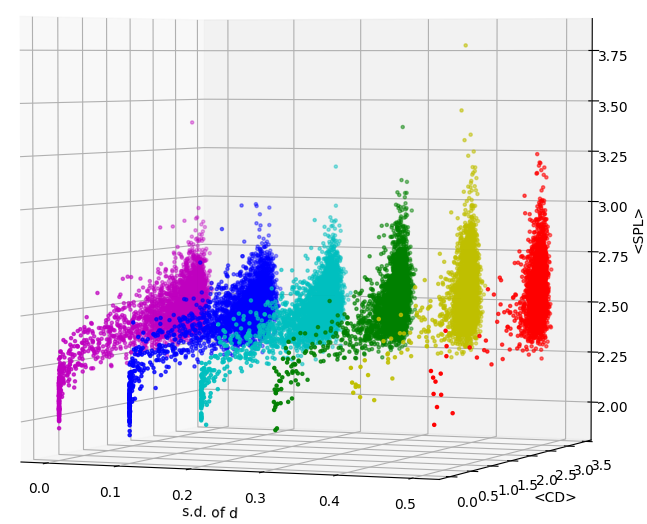
\includegraphics[width=.45\linewidth]{images/d cd spl 0.8 scc.png}}\par

    \subfloat[]{\label{}
    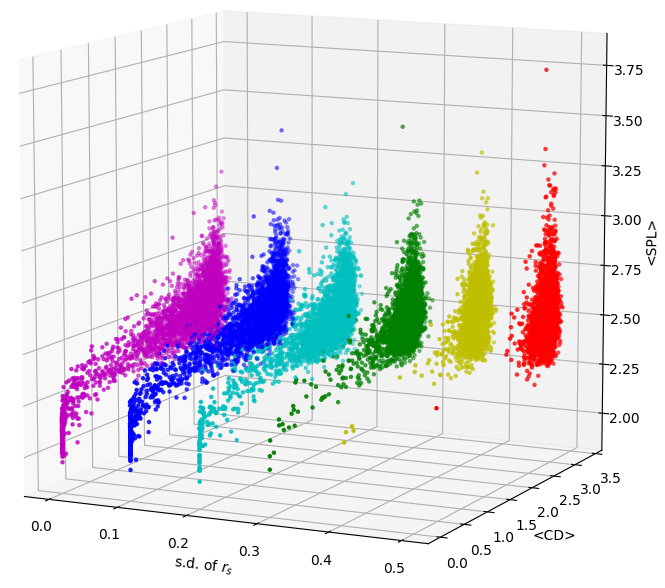
\includegraphics[width=.35\linewidth]{images/rs cd spl 0.8 scc redcued.png}}\hfill
    \subfloat[]{\label{}
    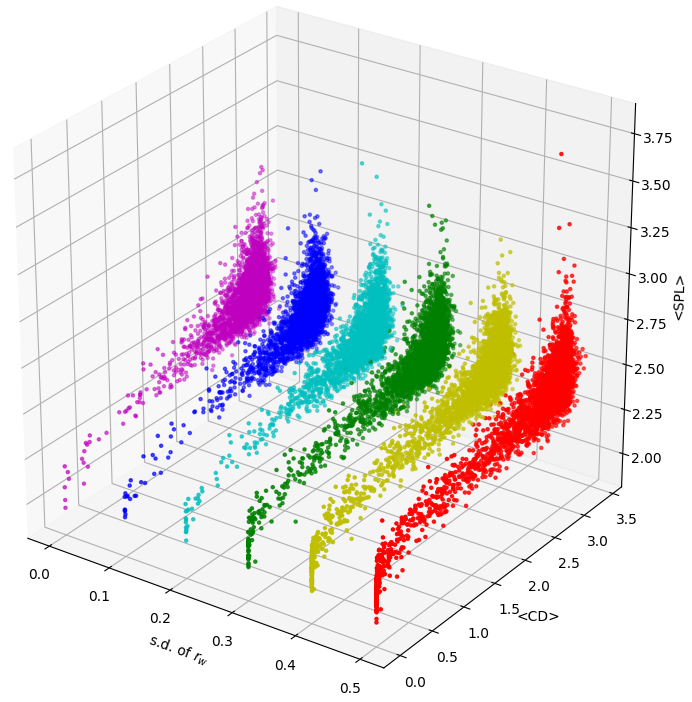
\includegraphics[width=.35\linewidth]{images/rw cd spl 0.8 scc reduced.png}}

    \caption{3D scatter plots showing the effect on $SPL_s$ and CD of each
    standard deviation of
    (a) $d$, (b) $r_s$ and (c)$r_w$. Each dot is the result of one simulation run, colored
    according to the standard deviation value.}
    \label{figure}
\end{figure}

\subsection{Linear Regression}

\begin{gather}\label{eq:reduced}
    <CD> ~ \thicksim ~ 2.28 + 1.73\sd + 1.82\sr - 2.20\sw -
                5.44\ds + 2.92\dw + 3.05\ssw \label{red1}\\
    <SPL_s> ~ \thicksim ~ 2.40 - 0.27\sd + 0.22\sr - 0.10 \sw -
                0.14\ds + 0.17\dw + 0.17\ssw \label{red2}
\end{gather}